%% $Id: overview.tex,v 1.17 2001/08/18 00:56:25 borning Exp $

\section{Overview of the UrbanSim Architecture}
\label{sec:overview}

To simulate an urban region, UrbanSim employs a collection of
interacting \emph{models}, representing different actors and
processes in the urban environment, such as residents, businesses,
land developers, and transportation networks.  Each model encodes
the behavior of agents in the simulation, as well as the objects
they operate upon, such as land parcels and buildings.  Objects
correlate directly with easily-identifiable objects in the real
world, making it easier to reason about their properties and
behaviors.  Agents can be shared across models, as can the objects
they operate upon.  Much more than other urban modeling systems,
the UrbanSim model is very disaggregate and has high data
requirements.  These requirements enable modeling of processes to
be done at a fine level, which allows use of detailed spatial data
in a manner not possible with more aggregate systems.  At the same
time, this makes the design and implementation of the system more
difficult from a software perspective.  Figure \ref{fig:USArch}
illustrates the software architecture of the UrbanSim system.

\begin{figure*}
\center \resizebox{0.75
\textwidth}{!}{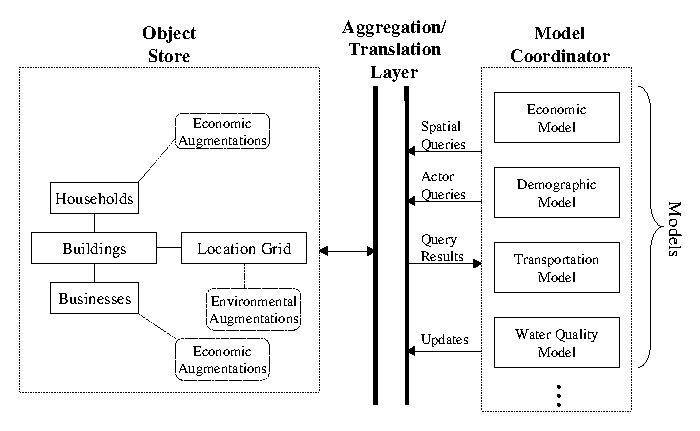
\includegraphics{USDiag1.eps}} \caption{UrbanSim
architecture} \label{fig:USArch}
\end{figure*}

%Figure~\ref{fig:USArch}: UrbanSim architecture.

In addition to the models, the other principal components of
UrbanSim are a \emph{model coordinator} that schedules models to
run and notifies them when data of interest have changed, an
\emph{object store} that holds the shared representations of
agents and other entities in the simulated world, and a
\emph{translation and aggregation layer} that performs a range of
data conversions to mediate between the Object Store and the
models.  The models do not communicate directly with each other;
rather, they communicate via shared data held in the Object Store,
mediated by the translation and aggregation layer.  This
extensible, modular architecture supports system evolution, in
particular replacing a model with a revised one, and creating and
integrating new models.  It allows models to define and share
common sets of objects that they all operate upon, via the Object
Store (regardless of the original source of the data), and also
allows them to monitor changes to data fields, providing a
convenient method for models to synchronize their actions.

A primary goal of this architecture is to move as much of the
software complexity out of the individual models and into the
supporting infrastructure as possible.  This supporting
infrastructure need be written just once, and can have the
attention of an expert programmer.  The models, on the other hand,
are both numerous and frequently changing due to rapidly evolving
theory, methods and modeling needs. Often, specifying them is
difficult, requiring considerable domain-specific expertise,
specialized data, and testing; the more one can relieve the model
designers of programming burdens the better, so that they can
concentrate on issues arising from the domain.

% LocalWords:  Exp UrbanSim USDiag eps noth borning pwaddell
